\documentclass[conference]{IEEEtran}
\IEEEoverridecommandlockouts
% The preceding line is only needed to identify funding in the first footnote. If that is unneeded, please comment it out.
\usepackage{cite}
\usepackage{amsmath,amssymb,amsfonts}
\usepackage{algorithmic}
\usepackage{graphicx}
\usepackage{textcomp}
\usepackage{xcolor}
\usepackage{soul}
\usepackage{booktabs}
\usepackage{multirow}
\def\BibTeX{{\rm B\kern-.05em{\sc i\kern-.025em b}\kern-.08em
    T\kern-.1667em\lower.7ex\hbox{E}\kern-.125emX}}
\pagestyle{plain}
\begin{document}

\title{Impact of German electricity market zone splitting on spatial distribution of charging demand of international battery-electric truck flow along the Scandinavian-Mediterranean corridor\\
{\footnotesize \textsuperscript{*}Note: Sub-titles are not captured in Xplore and
should not be used}
\thanks{Identify applicable funding agency here. If none, delete this.}
}

% \author{\IEEEauthorblockN{1\textsuperscript{st} Given Name Surname}
% \IEEEauthorblockA{\textit{dept. name of organization (of Aff.)} \\
% \textit{name of organization (of Aff.)}\\
% City, Country \\
% email address or ORCID}
% \and
% \IEEEauthorblockN{2\textsuperscript{nd} Given Name Surname}
% \IEEEauthorblockA{\textit{dept. name of organization (of Aff.)} \\
% \textit{name of organization (of Aff.)}\\
% City, Country \\
% email address or ORCID}
% \and
% \IEEEauthorblockN{3\textsuperscript{rd} Given Name Surname}
% \IEEEauthorblockA{\textit{dept. name of organization (of Aff.)} \\
% \textit{name of organization (of Aff.)}\\
% City, Country \\
% email address or ORCID}
% \and
% \IEEEauthorblockN{4\textsuperscript{th} Given Name Surname}
% \IEEEauthorblockA{\textit{dept. name of organization (of Aff.)} \\
% \textit{name of organization (of Aff.)}\\
% City, Country \\
% email address or ORCID}
% \and
% \IEEEauthorblockN{5\textsuperscript{th} Given Name Surname}
% \IEEEauthorblockA{\textit{dept. name of organization (of Aff.)} \\
% \textit{name of organization (of Aff.)}\\
% City, Country \\
% email address or ORCID}
% \and
% \IEEEauthorblockN{6\textsuperscript{th} Given Name Surname}
% \IEEEauthorblockA{\textit{dept. name of organization (of Aff.)} \\
% \textit{name of organization (of Aff.)}\\
% City, Country \\
% email address or ORCID}
% }

\maketitle

\begin{abstract}
This document is a model and instructions for \LaTeX.
This and the IEEEtran.cls file define the components of your paper [title, text, heads, etc.]. *CRITICAL: Do Not Use Symbols, Special Characters, Footnotes, 
or Math in Paper Title or Abstract.
\end{abstract}

\begin{IEEEkeywords}
component, formatting, style, styling, insert
\end{IEEEkeywords}

\section{Introduction}
\subsection{Motivation}

Across Europe, electricity market design is evolving from large, uniform bidding zones toward mechanisms that better reflect local pricing signals. This trend is driven by the need to address persistent grid congestion that arises when uniform wholesale prices fail to signal the true cost of electricity delivery across geographically diverse networks \cite{b_moretto2026, b_knorr2025}. As renewable generation---particularly wind power---concentrates in specific regions, the mismatch between generation and demand creates systematic congestion patterns that uniform pricing cannot resolve, leading to costly redispatch interventions and inefficient investment signals.

One of the most prominent instances of this debate is the potential splitting of the German electricity market zone. Germany currently operates as a single bidding zone despite significant structural congestion along its North--South axis: wind-rich northern regions generate surplus electricity that must be transmitted to demand-heavy southern industrial centers. This discussion has been ongoing for over a decade and is driven by several compounding factors. First, the accelerated phase-out of nuclear power (completed in 2023) and the planned phase-out of coal-fired generation have removed large dispatchable capacities predominantly located in Southern Germany~\cite{b_fraunholz2021}. Second, the expansion of wind power---the backbone of Germany's renewable energy strategy---is geographically concentrated in the North, widening the spatial imbalance between generation and load~\cite{b_trepper2015, b_fraunholz2021}. Third, the transmission grid expansion needed to bridge this gap, including major HVDC corridors such as S\"udLink and S\"udOstLink, has been repeatedly delayed~\cite{b_fraunholz2021, b_knorr2025}. As a consequence, redispatch volumes and costs have increased substantially, reaching 34~TWh and EUR~3.1~billion in Germany in 2023~\cite{b_knorr2025}. In response, the EU~Commission mandated a Bidding Zone Review (BZR) as part of the Clean Energy Package, in which ACER proposed alternative configurations for the German-Luxembourgish zone, including a North--South split~\cite{b_knorr2025, b_moretto2026}. The resulting price effects have been studied extensively: Trepper et al.~\cite{b_trepper2015} find average price differences of 1.55--3.56~EUR/MWh between a Northern and Southern zone; Fraunholz et al.~\cite{b_fraunholz2021} report relative day-ahead price differentials of 5--18\% depending on the time horizon; and Kn\"orr et al.~\cite{b_knorr2025} estimate an average spread of approximately 4.77~EUR/MWh. A precedent already exists: the German--Austrian bidding zone was split in October 2018 due to persistent congestion on the interconnectors~\cite{b_hurta2022}. Moreover, the effects of a German zone split would not be confined to Germany---\O stergaard et al.~\cite{b_ostergaard2025} show that the current single German zone inflates electricity prices in neighboring Denmark, and Emelianova et al.~\cite{b_emelianova2025} highlight the cross-border redistributive consequences of such market reconfigurations.

Simulation studies have quantified these effects across multiple dimensions. On the \emph{electricity market} side, Trepper et al.~\cite{b_trepper2015} show that a North--South split reduces redispatch volumes significantly but produces considerable distributional effects: consumers in the Northern zone benefit from lower prices while those in the South face higher costs, and the authors note that persistently higher prices in Southern Germany could incentivize either generation expansion or demand migration to cheaper regions. Fraunholz et al.~\cite{b_fraunholz2021} extend this analysis to the long term and find that the split strongly affects \emph{generation investment}: substantially more new conventional capacity is built in the higher-priced Southern zone, while storage investments shift to the wind-rich North. They also report a negative overall welfare effect for Germany, driven by the limited transfer capacity between zones leading to a less efficient market outcome---though neighboring countries may benefit from the reconfiguration. Critically, they find that the optimal zonal configuration for the base year~2020 becomes outdated by~2035 due to dynamic effects of grid extension, renewable expansion, and new power plant investments, cautioning that static zone definitions can create path dependencies. On a broader European scale, Moretto and Pollitt~\cite{b_moretto2026} compare zonal pricing systems across Norway, Sweden, Italy, Australia, Texas, and California, finding that while zonal configurations can improve transparency and investment signals, their effectiveness is highly context-dependent and requires periodic reassessment. Beyond the electricity sector itself, the effects of zone configurations cascade into \emph{end-use sectors} that depend on electricity as an input. \O stergaard et al.~\cite{b_ostergaard2025} demonstrate that the current single German zone artificially inflates electricity prices in neighboring Denmark, directly undermining the feasibility of electrification across heating (power-to-heat), transportation, and industry---sectors central to the Danish energy transition. Emelianova et al.~\cite{b_emelianova2025} highlight that cross-border market reconfigurations create substantial redistributive consequences, with consumers and energy-intensive industries in exporting regions (such as Sweden's southern bidding zone) facing price increases that have triggered political opposition to interconnector projects. Similarly, Hurta et al.~\cite{b_hurta2022} show that the 2018 German--Austrian zone split altered the investment viability of grid-scale battery storage in Austria. At the most granular level, Cho et al.~\cite{b_cho2015} find that regionally varying electricity prices affect demand differently across economic sectors---manufacturing and retail demand respond near-proportionally to price changes, while agricultural and residential uses are largely price-inelastic---underscoring that the spatial redistribution of electricity costs has sector-specific consequences.

A consumer sector that is rarely discussed in this context is \emph{commercial road transport}. While the role of charging costs in the optimal operation of battery-electric trucks along selected routes has been studied---including how these costs vary with intra-day electricity price volatility and between discrete charger types such as depot slow charging versus fast charging en route~\cite{b_noll2022}---the effect of price differences \emph{across electricity market zones} on charging demand allocation over larger geographic scopes has yet to be addressed. An exception is the work by Pagnier et al.~\cite{b_pagnier2026}, who plan the decarbonization of the freight transport sector across all transport modes within Norway while explicitly considering the Norwegian electricity price zones, finding a relevant relationship between the optimal location of battery-electric truck adoption and the resulting zonal electricity price. Simultaneously, Noll et al.~\cite{b_noll2022} show that charging costs---which are largely determined by the local electricity price---significantly impact the cost competitiveness between internal combustion engine and battery-electric drivetrains, with total cost of ownership differing substantially between European countries. Lanz et al.~\cite{b_lanz2022} also highlight the electricity price component as a major driver of charging costs, albeit for passenger cars, confirming the sensitivity of electric vehicle economics to local electricity pricing.

An added dimension in the transport sector, compared with stationary consumers such as industry or heating, is that transport consumers are \emph{mobile}: long-haul trucks travel across multiple regions and, for international freight, across national borders and electricity market zones. This mobility creates an opportunity---when charging is optimized over the route---to exploit spatial price differentials by shifting charging demand toward regions with lower electricity costs, thereby improving cost competitiveness. It also means that a zone split in one country (here, Germany) can redistribute charging loads not only within that country but along the entire transit corridor.

Three consequences of a German zone split are particularly relevant for the freight transport sector but have not been studied. First, by altering the relative cost competitiveness of battery-electric versus diesel trucks, a zone split can \emph{accelerate or delay electrification} along routes transiting through Germany, directly affecting CO$_2$ emissions on German highways---an effect that depends on whether the cheaper Northern zone or the more expensive Southern zone dominates the route. Second, since trucks can shift where they charge along a route, a price differential between zones will \emph{redistribute charging demand spatially}, concentrating it in cheaper regions while depleting it in more expensive ones---with implications for grid planning and electricity demand forecasting in both zones. Third, as Fraunholz et al.~\cite{b_fraunholz2021} caution for generation investment, the \emph{timing} of the zone split matters: if charging infrastructure is built under unified prices and the split is introduced later, regions that lose charging demand (the more expensive Southern zone) may face \emph{stranded or underutilized infrastructure}---an irreversible investment that cannot be relocated.

\subsection{Research Objective}
This leads to the following research question: \textbf{How does a splitting of the German electricity market zone affect (1)~CO$_2$ emissions from freight transport on German highways, (2)~the spatial distribution of truck charging demand between Northern and Southern Germany, and (3)~the risk of stranded charging infrastructure when the split is introduced at different points in time?}

We address this by simulating a market split via expected electricity price levels under different conditions of the split (spread magnitude and timing), deriving location-specific charging costs, and modeling the long-term demand response with a linear program for cost-optimal multi-year fleet turnover and charging demand allocation along origin-destination truck flows on the Scandinavian-Mediterranean corridor.

\section{Methodology and Data}

\subsection{German market zone splitting}

We simulate the impact of a hypothetical German electricity market zone split by constructing a scenario matrix that varies two dimensions: (i)~the \emph{magnitude} of the North--South electricity price spread, and (ii)~the \emph{timing} of when the zone split takes effect. The scenario matrix is summarized in Table~\ref{tab:scenarios}.

\subsubsection{Scenario design}
A single \emph{baseline} scenario assumes a unified German price zone throughout the modeling horizon (2020--2060), corresponding to the current market design. Six zone-split scenarios are constructed by combining three spread levels with two implementation timings (from~2032 and from~2040).

\textbf{Price spread levels.}
The price differential between the North and South German zones is applied as a symmetric, relative adjustment to the baseline wholesale electricity price at each node:
\begin{itemize}
    \item \textbf{Low (5\%):} North $-2.5\%$, South $+2.5\%$ --- conservative, based on early estimates by Trepper et al.~\cite{b_trepper2015}
    \item \textbf{Mid (10\%):} North $-5\%$, South $+5\%$ --- central estimate, consistent with Kn\"orr et al.~\cite{b_knorr2025} and Fraunholz et al.~\cite{b_fraunholz2021}
    \item \textbf{High (20\%):} North $-10\%$, South $+10\%$ --- upper bound, reflecting early-period spreads in Fraunholz et al.~\cite{b_fraunholz2021}
\end{itemize}
Using a relative (percentage-based) differential ensures that the absolute price spread scales with the price level: larger in early years when wholesale prices are higher, and smaller as prices decline with renewable energy expansion.\footnote{For the High (20\%) scenario, the resulting fast-charging price spread (including CPO markup) between North and South Germany is approximately 5.2~ct/kWh in 2030 and 2.9~ct/kWh in 2040; for Mid (10\%) it is 2.6 and 1.5~ct/kWh; for Low (5\%) it is 1.3 and 0.7~ct/kWh, respectively. For a BEV truck consuming $\sim$1.2~kWh/km over a typical $\sim$600~km German transit segment, the High scenario translates to a cost difference of roughly EUR~37 per trip in 2030 and EUR~21 in 2040 between charging entirely in the North versus entirely in the South.}

\textbf{Implementation timing.}
The zone split takes effect in one of three years:
\begin{itemize}
    \item \textbf{From 2020:} split applies from the beginning of the modeling horizon
    \item \textbf{From 2032:} prices remain unified until 2031; split from 2032 onward
    \item \textbf{From 2040:} prices remain unified until 2039; split from 2040 onward
\end{itemize}
Before the split year, all German nodes retain the baseline (unified) electricity price. This dimension captures the policy uncertainty around \emph{when} such a reform might be implemented, and whether early versus late splitting has different effects on the already-established truck fleet and charging infrastructure.

\textbf{Zone definition.}
Germany is divided into two zones following the TSO boundary convention used in Trepper et al.~\cite{b_trepper2015} and Fraunholz et al.~\cite{b_fraunholz2021}:
\begin{itemize}
    \item \textbf{North} (50Hertz + TenneT-North): wind-rich regions with lower marginal generation costs (Lower Saxony, Schleswig-Holstein, Mecklenburg-Vorpommern, Brandenburg, Berlin, Saxony, Saxony-Anhalt, Thuringia, Bremen, Hamburg)
    \item \textbf{South} (Amprion + TransnetBW + Bavaria): demand-heavy regions with higher marginal costs (NRW, Hesse, Rhineland-Palatinate, Saarland, Baden-W\"urttemberg, Bavaria)
\end{itemize}

\begin{table}[htbp]
\caption{Scenario matrix: 1 baseline + 6 zone-split scenarios}
\label{tab:scenarios}
\begin{center}
\begin{tabular}{l c c}
\toprule
 & \multicolumn{2}{c}{\textbf{Split timing}} \\
\cmidrule(lr){2-3}
\textbf{Spread} & From 2032 & From 2040 \\
\midrule
Baseline (0\%) & \multicolumn{2}{c}{DE\_unified (reference)} \\
\midrule
Low (5\%)  & \checkmark & \checkmark \\
Mid (10\%) & \checkmark & \checkmark \\
High (20\%) & \checkmark & \checkmark \\
\bottomrule
\end{tabular}
\end{center}
\end{table}

\subsubsection{Electricity prices and charging costs}
Baseline wholesale electricity prices are taken from the \textbf{Go~RES} scenario of GENeSYS-MOD~\cite{b_genesys}, which assumes ambitious renewable energy expansion in line with the EU's Green Deal targets. This scenario was selected because it represents a central pathway with high renewable penetration---precisely the conditions under which North--South price differentials in Germany are expected to be most pronounced due to the geographic concentration of wind power in the North. Go~RES provides node-level annual wholesale electricity prices for 2020--2060 across all corridor countries (NO, FI, SE, DK, DE, AT, IT). For zone-split scenarios, the German prices are adjusted as described above: for each German node, the wholesale price is multiplied by $(1 - \delta/2)$ in the North zone or $(1 + \delta/2)$ in the South zone, where $\delta$ is the relative spread (5\%, 10\%, or 20\%). This adjustment is only applied from the split year onward; earlier years retain the unified price.

\hl{Local charging costs are composed of: wholesale electricity price, network charges (grid fees), CPO markup, and charging infrastructure investment costs. Describe each component and how they vary spatially. Include map showing two snapshots of charging cost landscape.}

Fig.~\ref{fig:elec_prices} shows the resulting electricity charging prices (including CPO markup) for all four spread levels with the earliest timing (from~2032). The North--South differential is clearly visible for the Mid and High spread cases, while non-German countries remain unaffected.

\begin{figure}[htbp]
\centerline{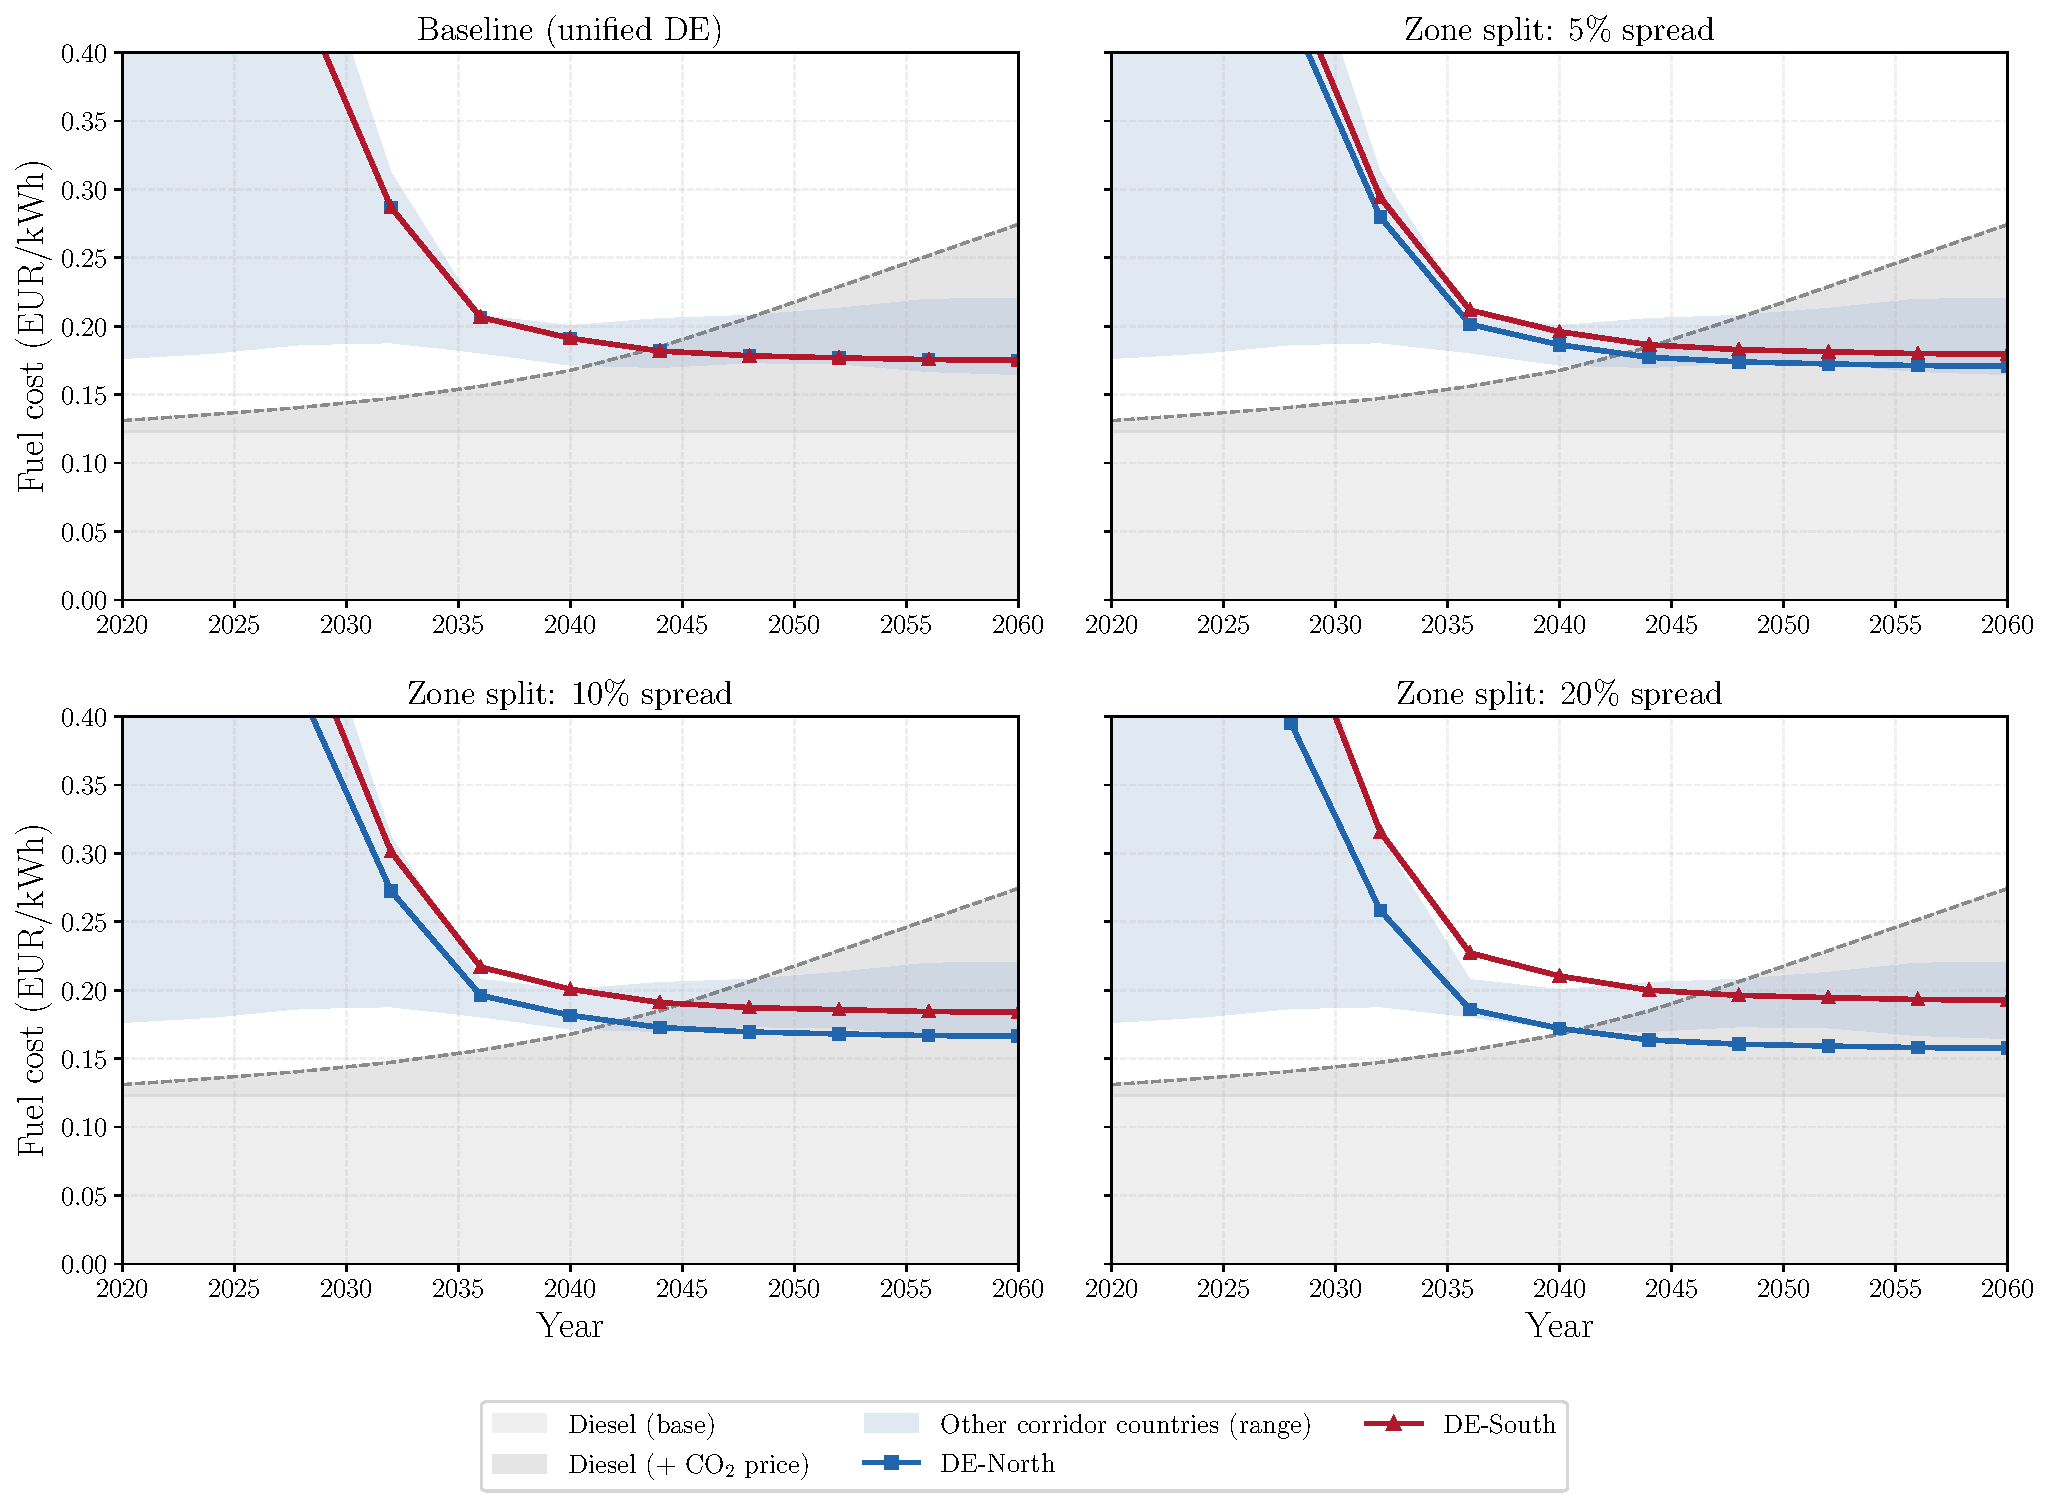
\includegraphics[width=\columnwidth]{eem_electricity_prices_by_country_4scenarios.pdf}}
\caption{Fast-charging electricity prices by country and German zone for the four spread levels (split from 2032). Gray areas show diesel cost (base and including CO$_2$ price). DE-North (squares) and DE-South (triangles) diverge with increasing spread.}
\label{fig:elec_prices}
\end{figure}

\subsection{Cost-optimization of fleet turnover and charging demand allocation}

The spatial allocation of charging demand and fleet composition is determined by a linear program that minimizes total discounted system cost over the horizon 2020--2060 with a 4-year time step. The model, TransComp~\cite{b_transcomp}, is formulated as a network design problem and determines, for each OD pair and period, the cost-optimal mix of ICEV and BEV trucks, the spatial allocation of charging energy along routes, and the required charging infrastructure investments. Table~\ref{tab:nomenclature} summarizes the key notation.

\begin{table}[htbp]
\caption{Key notation}
\label{tab:nomenclature}
\begin{center}
\footnotesize
\begin{tabular}{@{}ll@{}}
\toprule
\multicolumn{2}{l}{\textbf{Sets}} \\
$y \in \mathcal{Y}$ & modeled years \\
$r \in \mathcal{R}$ & origin-destination pairs \\
$t \in \mathcal{T}$ & drivetrain technologies (ICEV, BEV) \\
$g \in \mathcal{G}$ & vehicle generation (purchase year) \\
$e \in \mathbf{E}_r$ & geographic locations along route $r$ \\
\midrule
\multicolumn{2}{l}{\textbf{Decision variables}} \\
$f_{yrtg}$ & transport volume [t/a] \\
$h_{yrtg}$, $h^+_{yrtg}$ & fleet stock; new purchases \\
$s_{yrtge}$ & charged energy at location $e$ [kWh/a] \\
$soc_{yrtge}$ & state of charge at $e$ [kWh] \\
$q^+_{ye}$ & added charging infra.\ capacity [kW] \\
\midrule
\multicolumn{2}{l}{\textbf{Key parameters}} \\
$F_{yr}$ & freight demand [t/a] \\
$D^{\mathrm{spec}}_{tg}$ & specific energy consumption [kWh/km] \\
$Q^{\mathrm{batt}}_{tg}$ & battery/tank capacity [kWh] \\
$p^{\mathrm{fuel}}_{te}(y)$ & location-specific fuel price [EUR/kWh] \\
$\pi^{\mathrm{CO_2}}_e(y)$ & carbon price [EUR/tCO$_2$] \\
\bottomrule
\end{tabular}
\end{center}
\end{table}

\subsubsection{Objective function}
The objective minimizes the net present value of all costs:
\begin{equation} \label{equ:obj}
    \min_{\mathbf{x}}\; z = \sum_{y \in \mathcal{Y}} d_y \,\Delta \Big( C^{\mathrm{veh}}_y + C^{\mathrm{fuel}}_y + C^{\mathrm{toll}}_y + C^{\mathrm{travel}}_y + C^{\mathrm{charg}}_y \Big)
\end{equation}
where $d_y = (1+\rho)^{-(y-y_0)}$ is the discount factor and $\Delta$ is the period length (4~years). Vehicle costs $C^{\mathrm{veh}}$ include CAPEX of new purchases and age-dependent maintenance. Fuel costs $C^{\mathrm{fuel}}$ include location-specific energy prices and a carbon surcharge for fossil fuels: $\sum_{r,t,g,e} s_{yrtge} \cdot ( p^{\mathrm{fuel}}_{te}(y) + \varepsilon_t \cdot \pi^{\mathrm{CO_2}}_e(y))$. Toll costs $C^{\mathrm{toll}}$ are technology-differentiated distance-based road charges. Travel time costs $C^{\mathrm{travel}}$ monetize only the \emph{deviation} from baseline travel time (driving + mandatory breaks) using a value of time, so that charging during mandatory driver rest incurs no additional cost. Charging infrastructure costs $C^{\mathrm{charg}}$ cover CAPEX, O\&M, and grid connection charges for deployed capacity.

\subsubsection{Key constraints}

\textbf{Demand coverage.} All freight demand must be served:
\begin{equation}
    \sum_{t,g} f_{yrtg} = F_{yr} \quad \forall\, y, r
\end{equation}

\textbf{Fleet turnover.} The vehicle stock is tracked by generation through a stock-flow balance of existing vehicles, retirements (after fixed lifetime $\Lambda_{tg}$), and new purchases, capturing the fleet inertia that constrains the pace of technology transition.

\textbf{State of charge.} The battery state of charge is tracked spatially along each route:
\begin{equation}
    soc_{yrtge_{i}} = soc_{yrtge_{i-1}} + s_{yrtge_{i}} - D^{\mathrm{spec}}_{tg} \cdot L_{e_{i-1,i}} \cdot \frac{f_{yrtg}}{W_{tg}}
\end{equation}
with initial SOC set to $SOC^{init} \cdot Q^{\mathrm{batt}}_{tg}$ and a minimum final SOC constraint. The SOC must remain within $(0, Q^{\mathrm{batt}}_{tg})$ at all intermediate nodes, preventing stranding and ensuring feasibility of BEV operation. This constraint is the key mechanism through which electricity prices affect spatial charging allocation: the optimizer distributes charged energy $s$ along the route to minimize fuel cost subject to the battery capacity envelope.

\textbf{Charging infrastructure.} Installed capacity (initial + cumulative expansion) must meet peak demand at each location:
\begin{equation}
    Q^{\mathrm{charg}}_{e} + \sum_{y' \leq y} q^+_{y'e} \;\geq\; \gamma \sum_{r \in \mathcal{R}_e} \sum_{t,g} s_{yrtge} \quad \forall\, y, e
\end{equation}
where $\gamma$ converts annual energy to peak power demand. Infrastructure, once built, is irreversible---creating path dependencies when the zone split is introduced at different times.

\subsection{Traffic flow data}

The model operates on origin-destination (OD) freight flows at the NUTS-2 level along the Scandinavian-Mediterranean TEN-T corridor, covering Norway, Finland, Sweden, Denmark, Germany, Austria, and Italy. Freight volumes are derived from the ETISplus European freight transport database~\cite{b_speth2021}, which provides bilateral road freight tonnages between NUTS-2 regions. Routes are computed as shortest-path sequences of NUTS-2 regions over the highway network, and mandatory driver rest stops are allocated along each route following EU~Regulation~561/2006 (4.5~h maximum continuous driving time)~\cite{b_transcomp}.

Two route categories are included:
\begin{enumerate}
    \item \textbf{International routes passing through Germany:} cross-border OD pairs whose path transits through at least one German NUTS-2 region (e.g., IT$\leftrightarrow$DE, SE$\leftrightarrow$DE, IT$\leftrightarrow$SE via DE). International routes that bypass Germany entirely (e.g., AT$\leftrightarrow$IT, DK$\leftrightarrow$NO via SE) are excluded since they are unaffected by the German zone split and would produce identical results across all scenarios.
    \item \textbf{German domestic N--S routes:} OD pairs where both origin and destination are in Germany but in \emph{different} electricity market zones (North$\leftrightarrow$South). These routes are essential for the zone-splitting analysis because trucks traveling within Germany across the zone boundary can reallocate charging between cheaper (North) and more expensive (South) regions.
\end{enumerate}

All routes are subject to the following filters:
\begin{itemize}
    \item \textbf{Minimum path length:} 360~km (corresponding to $\sim$4.5~hours of driving at 80~km/h, i.e., one mandatory driver rest interval)
    \item \textbf{Minimum freight volume:} 500~tonnes/year in the base year
    \item \textbf{Transit through Germany:} only routes whose path passes through at least one German region
\end{itemize}
After filtering, the dataset contains approximately 1,787 international OD pairs transiting through Germany and 83 German cross-zone domestic OD pairs, for a total of $\sim$1,870 routes. The 249 international routes bypassing Germany (e.g., AT$\leftrightarrow$IT, Scandinavian intra-Nordic) are excluded to reduce computational cost without affecting results.

\section{Results}

\subsection{Route-level electrification shifts}

While the aggregate BEV fleet share remains nearly identical across all scenarios ($\sim$43.7\% at 2040), the zone split fundamentally reshapes \emph{which} routes electrify. Fig.~\ref{fig:violin} shows the distribution of route-level BEV share changes between the High~(20\%) from-2032 scenario and the baseline at~2040, disaggregated by corridor type. Routes are classified as \emph{North only} if their path passes exclusively through DE-North NUTS-2 regions, \emph{South only} if exclusively through DE-South, and \emph{cross-zonal} if through both.

North-only routes gain on average $+21$~pp in BEV share, with many routes shifting from $\sim$15\% to 100\% BEV---corresponding to approximately 1,230 additional tonnes transported by BEV trucks on these corridors. Conversely, South-only routes lose on average $-18$~pp, with $\sim$2,980~tonnes shifting back from BEV to ICEV. Cross-zonal routes show mixed effects (mean $+4$~pp), with 245~routes gaining and 100~losing more than 5~pp BEV share.

\begin{figure}[htbp]
\centerline{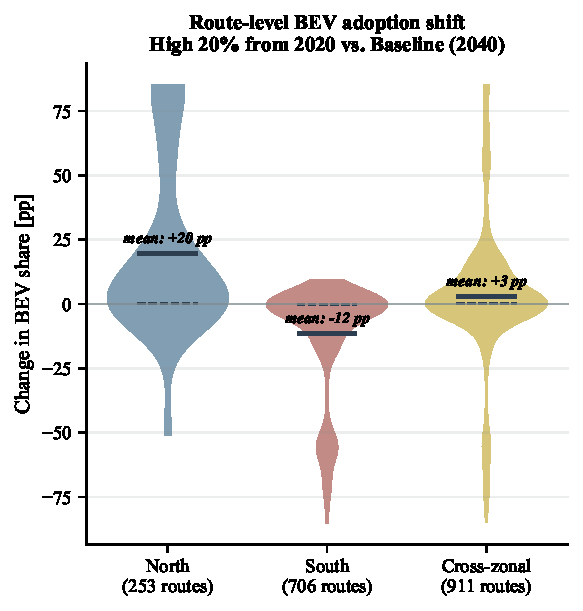
\includegraphics[width=0.85\columnwidth]{eem_route_bev_violin.pdf}}
\caption{Distribution of route-level BEV share changes (High 20\%, from 2032 vs.\ baseline) at 2040 by corridor type. Solid line: mean; dashed line: median. North-only routes gain BEV share while South-only routes lose it, despite identical aggregate fleet composition. \hl{needs a bottom axis}}
\label{fig:violin}
\end{figure}

\subsection{Spatial redistribution of charging demand}

\section{Conclusion and Future Work}

The zone split does not change the aggregate BEV fleet size but fundamentally reshapes \emph{where} charging demand arises, creating regional winners and losers along the Scandinavian--Mediterranean freight corridor. A promising extension is a \textbf{rolling-horizon} formulation: instead of a single-shot optimization over the full planning horizon, infrastructure investment decisions would be made with limited foresight. This would capture the risk of building charging capacity under one market-zone configuration (unified) that becomes underutilized if the zone split occurs later---providing a more realistic estimate of stranded infrastructure costs.

\section{Prepare Your Paper Before Styling}
Before you begin to format your paper, first write and save the content as a 
separate text file. Complete all content and organizational editing before 
formatting. Please note sections \ref{AA}--\ref{SCM} below for more information on 
proofreading, spelling and grammar.

Keep your text and graphic files separate until after the text has been 
formatted and styled. Do not number text heads---{\LaTeX} will do that 
for you.

\subsection{Abbreviations and Acronyms}\label{AA}
Define abbreviations and acronyms the first time they are used in the text, 
even after they have been defined in the abstract. Abbreviations such as 
IEEE, SI, MKS, CGS, ac, dc, and rms do not have to be defined. Do not use 
abbreviations in the title or heads unless they are unavoidable.

\subsection{Units}
\begin{itemize}
\item Use either SI (MKS) or CGS as primary units. (SI units are encouraged.) English units may be used as secondary units (in parentheses). An exception would be the use of English units as identifiers in trade, such as ``3.5-inch disk drive''.
\item Avoid combining SI and CGS units, such as current in amperes and magnetic field in oersteds. This often leads to confusion because equations do not balance dimensionally. If you must use mixed units, clearly state the units for each quantity that you use in an equation.
\item Do not mix complete spellings and abbreviations of units: ``Wb/m\textsuperscript{2}'' or ``webers per square meter'', not ``webers/m\textsuperscript{2}''. Spell out units when they appear in text: ``. . . a few henries'', not ``. . . a few H''.
\item Use a zero before decimal points: ``0.25'', not ``.25''. Use ``cm\textsuperscript{3}'', not ``cc''.)
\end{itemize}

\subsection{Equations}
Number equations consecutively. To make your 
equations more compact, you may use the solidus (~/~), the exp function, or 
appropriate exponents. Italicize Roman symbols for quantities and variables, 
but not Greek symbols. Use a long dash rather than a hyphen for a minus 
sign. Punctuate equations with commas or periods when they are part of a 
sentence, as in:
\begin{equation}
a+b=\gamma\label{eq}
\end{equation}

Be sure that the 
symbols in your equation have been defined before or immediately following 
the equation. Use ``\eqref{eq}'', not ``Eq.~\eqref{eq}'' or ``equation \eqref{eq}'', except at 
the beginning of a sentence: ``Equation \eqref{eq} is . . .''

\subsection{\LaTeX-Specific Advice}

Please use ``soft'' (e.g., \verb|\eqref{Eq}|) cross references instead
of ``hard'' references (e.g., \verb|(1)|). That will make it possible
to combine sections, add equations, or change the order of figures or
citations without having to go through the file line by line.

Please don't use the \verb|{eqnarray}| equation environment. Use
\verb|{align}| or \verb|{IEEEeqnarray}| instead. The \verb|{eqnarray}|
environment leaves unsightly spaces around relation symbols.

Please note that the \verb|{subequations}| environment in {\LaTeX}
will increment the main equation counter even when there are no
equation numbers displayed. If you forget that, you might write an
article in which the equation numbers skip from (17) to (20), causing
the copy editors to wonder if you've discovered a new method of
counting.

{\BibTeX} does not work by magic. It doesn't get the bibliographic
data from thin air but from .bib files. If you use {\BibTeX} to produce a
bibliography you must send the .bib files. 

{\LaTeX} can't read your mind. If you assign the same label to a
subsubsection and a table, you might find that Table I has been cross
referenced as Table IV-B3. 

{\LaTeX} does not have precognitive abilities. If you put a
\verb|\label| command before the command that updates the counter it's
supposed to be using, the label will pick up the last counter to be
cross referenced instead. In particular, a \verb|\label| command
should not go before the caption of a figure or a table.

Do not use \verb|\nonumber| inside the \verb|{array}| environment. It
will not stop equation numbers inside \verb|{array}| (there won't be
any anyway) and it might stop a wanted equation number in the
surrounding equation.

\subsection{Some Common Mistakes}\label{SCM}
\begin{itemize}
\item The word ``data'' is plural, not singular.
\item The subscript for the permeability of vacuum $\mu_{0}$, and other common scientific constants, is zero with subscript formatting, not a lowercase letter ``o''.
\item In American English, commas, semicolons, periods, question and exclamation marks are located within quotation marks only when a complete thought or name is cited, such as a title or full quotation. When quotation marks are used, instead of a bold or italic typeface, to highlight a word or phrase, punctuation should appear outside of the quotation marks. A parenthetical phrase or statement at the end of a sentence is punctuated outside of the closing parenthesis (like this). (A parenthetical sentence is punctuated within the parentheses.)
\item A graph within a graph is an ``inset'', not an ``insert''. The word alternatively is preferred to the word ``alternately'' (unless you really mean something that alternates).
\item Do not use the word ``essentially'' to mean ``approximately'' or ``effectively''.
\item In your paper title, if the words ``that uses'' can accurately replace the word ``using'', capitalize the ``u''; if not, keep using lower-cased.
\item Be aware of the different meanings of the homophones ``affect'' and ``effect'', ``complement'' and ``compliment'', ``discreet'' and ``discrete'', ``principal'' and ``principle''.
\item Do not confuse ``imply'' and ``infer''.
\item The prefix ``non'' is not a word; it should be joined to the word it modifies, usually without a hyphen.
\item There is no period after the ``et'' in the Latin abbreviation ``et al.''.
\item The abbreviation ``i.e.'' means ``that is'', and the abbreviation ``e.g.'' means ``for example''.
\end{itemize}
An excellent style manual for science writers is \cite{b7}.

\subsection{Authors and Affiliations}
\textbf{The class file is designed for, but not limited to, six authors.} A 
minimum of one author is required for all conference articles. Author names 
should be listed starting from left to right and then moving down to the 
next line. This is the author sequence that will be used in future citations 
and by indexing services. Names should not be listed in columns nor group by 
affiliation. Please keep your affiliations as succinct as possible (for 
example, do not differentiate among departments of the same organization).

\subsection{Identify the Headings}
Headings, or heads, are organizational devices that guide the reader through 
your paper. There are two types: component heads and text heads.

Component heads identify the different components of your paper and are not 
topically subordinate to each other. Examples include Acknowledgments and 
References and, for these, the correct style to use is ``Heading 5''. Use 
``figure caption'' for your Figure captions, and ``table head'' for your 
table title. Run-in heads, such as ``Abstract'', will require you to apply a 
style (in this case, italic) in addition to the style provided by the drop 
down menu to differentiate the head from the text.

Text heads organize the topics on a relational, hierarchical basis. For 
example, the paper title is the primary text head because all subsequent 
material relates and elaborates on this one topic. If there are two or more 
sub-topics, the next level head (uppercase Roman numerals) should be used 
and, conversely, if there are not at least two sub-topics, then no subheads 
should be introduced.

\subsection{Figures and Tables}
\paragraph{Positioning Figures and Tables} Place figures and tables at the top and 
bottom of columns. Avoid placing them in the middle of columns. Large 
figures and tables may span across both columns. Figure captions should be 
below the figures; table heads should appear above the tables. Insert 
figures and tables after they are cited in the text. Use the abbreviation 
``Fig.~\ref{fig}'', even at the beginning of a sentence.

\begin{table}[htbp]
\caption{Table Type Styles}
\begin{center}
\begin{tabular}{|c|c|c|c|}
\hline
\textbf{Table}&\multicolumn{3}{|c|}{\textbf{Table Column Head}} \\
\cline{2-4} 
\textbf{Head} & \textbf{\textit{Table column subhead}}& \textbf{\textit{Subhead}}& \textbf{\textit{Subhead}} \\
\hline
copy& More table copy$^{\mathrm{a}}$& &  \\
\hline
\multicolumn{4}{l}{$^{\mathrm{a}}$Sample of a Table footnote.}
\end{tabular}
\label{tab1}
\end{center}
\end{table}

\begin{figure}[htbp]
\centerline{
\includegraphics{fig1.png}}
\caption{Example of a figure caption.}
\label{fig}
\end{figure}

Figure Labels: Use 8 point Times New Roman for Figure labels. Use words 
rather than symbols or abbreviations when writing Figure axis labels to 
avoid confusing the reader. As an example, write the quantity 
``Magnetization'', or ``Magnetization, M'', not just ``M''. If including 
units in the label, present them within parentheses. Do not label axes only 
with units. In the example, write ``Magnetization (A/m)'' or ``Magnetization 
\{A[m(1)]\}'', not just ``A/m''. Do not label axes with a ratio of 
quantities and units. For example, write ``Temperature (K)'', not 
``Temperature/K''.

\section*{Acknowledgment}

The preferred spelling of the word ``acknowledgment'' in America is without 
an ``e'' after the ``g''. Avoid the stilted expression ``one of us (R. B. 
G.) thanks $\ldots$''. Instead, try ``R. B. G. thanks$\ldots$''. Put sponsor 
acknowledgments in the unnumbered footnote on the first page.

\section*{References}

Please number citations consecutively within brackets \cite{b1}. The 
sentence punctuation follows the bracket \cite{b2}. Refer simply to the reference 
number, as in \cite{b3}---do not use ``Ref. \cite{b3}'' or ``reference \cite{b3}'' except at 
the beginning of a sentence: ``Reference \cite{b3} was the first $\ldots$''

Number footnotes separately in superscripts. Place the actual footnote at 
the bottom of the column in which it was cited. Do not put footnotes in the 
abstract or reference list. Use letters for table footnotes.

Unless there are six authors or more give all authors' names; do not use 
``et al.''. Papers that have not been published, even if they have been 
submitted for publication, should be cited as ``unpublished'' \cite{b4}. Papers 
that have been accepted for publication should be cited as ``in press'' \cite{b5}. 
Capitalize only the first word in a paper title, except for proper nouns and 
element symbols.

For papers published in translation journals, please give the English 
citation first, followed by the original foreign-language citation \cite{b6}.

\begin{thebibliography}{00}
\bibitem{b_trepper2015} K. Trepper, M. Bucksteeg, and C. Weber, ``Market splitting in Germany -- new evidence from a three-zone stochastic electricity market model,'' \emph{Energy Policy}, vol.~87, pp. 199--215, 2015.
\bibitem{b_fraunholz2021} C. Fraunholz, K. Hladik, R. Kraft, D. Kern\-er, and W. Fichtner, ``On the long-term efficiency of market splitting in Germany,'' \emph{Energy Policy}, vol.~149, 111833, 2021.
\bibitem{b_knorr2025} M. Kn\"orr, C. Fraunholz, and W. Fichtner, ``Impacts of German bidding zone configurations on the European electricity market,'' arXiv:2403.09265v6, 2025.
\bibitem{b_zinke2023} J. Zinke, ``Bidding zone review: implications for Germany and Europe,'' EWI Working Paper 23/07, 2023.
\bibitem{b_genesys} H. Gardian, L. Hering, and P.-Y. Oei, ``GENeSYS-MOD -- open-source energy system model,'' 2024. [Online]. Available: https://git.tu-berlin.de/genesysmod
\bibitem{b_martin2024} J. Martin \emph{et al.}, ``Total cost of ownership and infrastructure requirements for long-haul battery-electric trucks in Europe,'' \emph{Transport Policy}, 2024.
\bibitem{b_moretto2026} M. Moretto and M. G. Pollitt, ``How many zones should an electricity market have? A cross-country perspective on bidding zone design,'' \emph{Energy Policy}, vol.~210, 115030, 2026.
\bibitem{b_hurta2022} A. Hurta, M. \v{Z}ilka, and F. Freiberg, ``Impact of the splitting of the German--Austrian electricity bidding zone on investment in a grid-scale battery energy storage system,'' \emph{Energy Reports}, vol.~8, pp. 12045--12062, 2022.
\bibitem{b_ostergaard2025} P. A. \O stergaard, A. N. Andersen, and F. D. Nielsen, ``Market zones and electrification -- A case study on the impact of market zone configuration on power-to-heat,'' \emph{Renewable and Sustainable Energy Reviews}, vol.~219, 115865, 2025.
\bibitem{b_emelianova2025} P. Emelianova, P. Hoffmann-Willers, and O. Ruhnau, ``Redistribution through cross-border electricity trade: How to achieve Pareto improvement?'' EWI Working Paper No.~25/11, 2025.
\bibitem{b_cho2015} S.-H. Cho, T. Kim, H.~J. Kim, K. Park, and R.~K. Roberts, ``Regionally-varying and regionally-uniform electricity pricing policies compared across four usage categories,'' \emph{Energy Economics}, vol.~49, pp. 182--191, 2015.
\bibitem{b_noll2022} B. Noll, S. del Val, T.~S. Schmidt, and B. Steffen, ``Analyzing the competitiveness of low-carbon drive-technologies in road-freight: A total cost of ownership analysis in Europe,'' \emph{Applied Energy}, vol.~306, 118079, 2022.
\bibitem{b_pagnier2026} C. Pagnier, S.~J.~S. Bakker, and P. Seljom, ``Decarbonizing freight transport: A quantitative framework linking energy system and freight transport models,'' \emph{Transportation Research Part D: Transport and Environment}, vol.~2026, 105114, 2026.
\bibitem{b_lanz2022} L. Lanz, B. Noll, T.~S. Schmidt, and B. Steffen, ``Comparing the levelized cost of electric vehicle charging options in Europe,'' \emph{Nature Communications}, vol.~13, no.~1, 5277, 2022.
\bibitem{b_speth2021} D. Speth, V. Sauter, P. Pl\"otz, and T. Signer, ``Synthetic European road freight transport flow data (ETISplus),'' Mendeley Data, V2, 2021. doi: 10.17632/s2f3k79554.2.
\bibitem{b_transcomp} A.~M. Golab, H. Gardian, P.-Y. Oei, and T.~S. Schmidt, ``TransComp: An optimization model for the transition to low-emission freight transport,'' 2025. [Online]. Available: https://github.com/antoniamgolab/iDesignRES\_transcompmodel
\end{thebibliography}

\appendix
\section{Vehicle Cost and Technical Assumptions}

Table~\ref{tab:vehicle_assumptions} summarizes the key cost and technical parameters for the two drivetrain technologies considered in this study.

\begin{table}[htbp]
\caption{Vehicle cost and technical assumptions}
\label{tab:vehicle_assumptions}
\begin{center}
\footnotesize
\begin{tabular}{@{}l l c c@{}}
\toprule
\textbf{Parameter} & \textbf{Unit} & \textbf{ICEV} & \textbf{BEV} \\
\midrule
\multicolumn{4}{l}{\textit{Capital cost (CAPEX)}} \\
\quad 2020 & kEUR & 169 & 550 \\
\quad 2030 & kEUR & 192 & 239 \\
\quad 2040 & kEUR & 192 & 218 \\
\midrule
\multicolumn{4}{l}{\textit{Operating cost}} \\
\quad Maintenance & kEUR/a & 20.7 & 14.4 \\
\quad Toll & EUR/km & 0.100 & 0.036 \\
\midrule
\multicolumn{4}{l}{\textit{Energy}} \\
\quad Spec.\ consumption 2020 & kWh/km & 3.64 & 2.06 \\
\quad Spec.\ consumption 2040 & kWh/km & 2.40 & 1.29 \\
\quad Tank / battery capacity & kWh & 5{,}529 & 1{,}187 \\
\quad Diesel price & EUR/kWh & \multicolumn{2}{c}{0.123 (constant)} \\
\quad CO$_2$ emission factor & gCO$_2$/kWh & 266 & 0 \\
\midrule
\multicolumn{4}{l}{\textit{Other}} \\
\quad Payload capacity & t & 13.6 & 10.9 \\
\quad Vehicle lifetime & a & 12 & 12 \\
\quad Annual mileage & km/a & \multicolumn{2}{c}{136{,}750} \\
\quad Discount rate & -- & \multicolumn{2}{c}{5\%} \\
\quad Value of time & EUR/h & \multicolumn{2}{c}{30} \\
\bottomrule
\end{tabular}
\end{center}
\end{table}

\end{document}
